%\begin{frame}{Opgave 3: Adaptiv kvadraturregler}
%    Forklar idéen i en sammensat adaptiv kvadraturregel.
%\end{frame}

\begin{frame}{Adaptiv kvadraturregler}
    Idéen i de adaptive kvadraturregler omhandler, hvordan en funktion kan behandles, når der ikke kan udvælges punkter til underinddeling på forhånd. Eksempelvis hvis funktionen ikke er kendt, men funktionsværdien kendes for en mængde af punkter. Der findes to primære måder at lave disse underinddelinger på. 
    \begin{itemize}
        \item 1. Der vælges et antal $N$ underindelinger af det oprindlige interval af formen $\left [  x_k, x_{k+1} \right ]$, hvor $a=x_0<x_1<x_2<\ldots<x_N$ herefter anvendes den sammensatte simpsons regel beskrevet i opgave 3 hvor antallet af underintervaller i de oprindelige $N$ gennemgår kontinuær fordobling.
        \item 2. Den anden måde benytter ligeledes den sammensatte simpsonsregel her på intervallet, denne udføres igen på de nye delintervaller samt på begge halvdele af disse, såfremt man er inden for den ønskede nøjagtighed for et givet interval accepteres dette som delresultat og der arbejdes nu med næste delinterval. Dette gentages indtil alle delintervaller er opdelt i et antal intervaller, der bringer det inden for den ønskede fejl.
    \end{itemize}
\end{frame}
%
%
%
\begin{frame}{Julie er et dejligt mennekse xD}
\phantom{H} \\
\centering
%
%%%%%%%%%%%%%%%%%%%%%%%%%%%%%%%%
%%% Flot graf alla Julie     %%%
%%%%%%%%%%%%%%%%%%%%%%%%%%%%%%%%
%
{\small
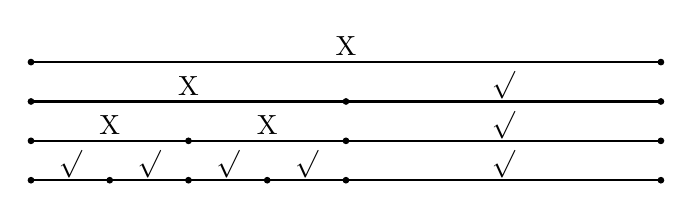
\begin{tikzpicture}[scale=1]
%
\draw[thick] (0,0) -- (8,0);
\filldraw [black] (0,0) circle (1pt);
\filldraw [black] (1,0) circle (1pt);
\filldraw [black] (2,0) circle (1pt);
\filldraw [black] (3,0) circle (1pt); 
\filldraw [black] (4,0) circle (1pt);
\filldraw [black] (8,0) circle (1pt); 
\node at (0.5,0.2) (){$\mathcal{p}$};
\node at (1.5,0.2) (){$\mathcal{p}$};
\node at (2.5,0.2) (){$\mathcal{p}$};
\node at (3.5,0.2) (){$\mathcal{p}$};
\node at (6,0.2) (){$\mathcal{p}$}; 
%
\draw[thick] (0,0.5) -- (8,0.5);
\filldraw [black] (0,0.5) circle (1pt);
\filldraw [black] (2,0.5) circle (1pt); 
\filldraw [black] (4,0.5) circle (1pt); 
\filldraw [black] (8,0.5) circle (1pt); 
\node at (1,0.7) (){X};
\node at (3,0.7) (){X};
\node at (6,0.7) (){$\mathcal{p}$}; 
%
\draw[thick] (0,1) -- (8,1);
\filldraw [black] (0,1) circle (1pt); 
\filldraw [black] (4,1) circle (1pt); 
\filldraw [black] (8,1) circle (1pt);
\node at (2,1.2) (){X};
\node at (6,1.2) (){$\mathcal{p}$};
%
\draw[thick] (0,1.5) -- (8,1.5);
\filldraw [black] (0,1.5) circle (1pt); 
\filldraw [black] (8,1.5) circle (1pt); 
\node at (4,1.7) (){X};
%
\end{tikzpicture}
}
\end{frame}